\documentclass[
  tikz,
  % ── protect the whole command ────────────────────────
  convert={
    outext=.svg,                   
    command=\unexpanded{
        "C:/Program Files/Inkscape/bin/inkscape.exe" -z \infile\space --export-type\detokenize{=}svg --export-filename\detokenize{=}\outfile\space 
    }                             
  },
  multi=false   
]{standalone}

\usepackage{pgfplots}
\pgfplotsset{compat=1.18}
\usepgfplotslibrary{groupplots}


\begin{document}

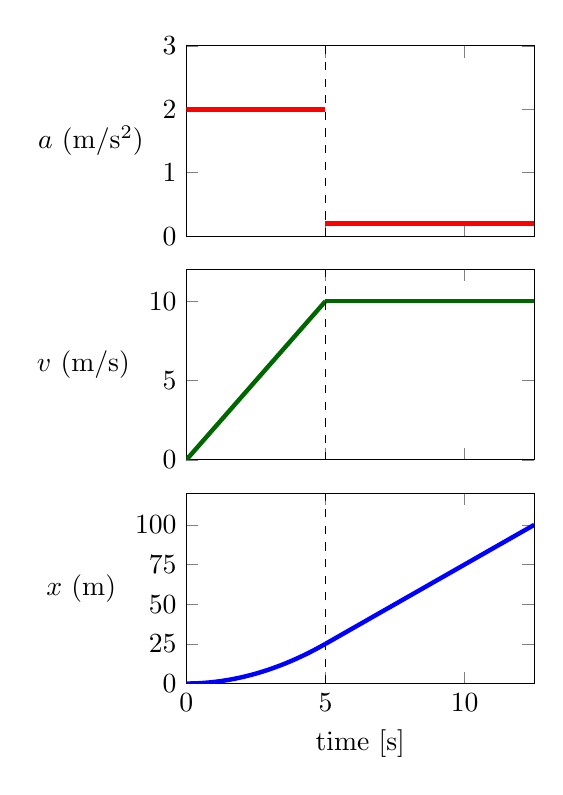
\begin{tikzpicture}[]
\begin{groupplot}[
    group style={
        group size=1 by 3, % Arrange plots in a single column
        vertical sep=12pt, % Remove vertical spacing between plots
        x descriptions at=edge bottom, % Place x-axis description only at the bottom plot
    },
    width=6cm, % Set width of each plot
    height=4cm, % Set height of each plot
    xlabel={time [s]},
    anchor=center,
    ylabel style={rotate=-90},
]

\nextgroupplot[xmin=0,xmax=12.5,ymin=0, ymax=3,ytick={0,1,2,3},ylabel={$a$ (m/s$^2$)} ]
\addplot[mark=none, red, ultra thick,domain=0:5, variable=t] {2};
\addplot[mark=none, red, ultra thick,domain=5:12.5, variable=t] {0.2};
\draw[dashed] (axis cs:5,0) -- (axis cs:5,3);


\nextgroupplot[xmin=0,xmax=12.5,ymin=0, ymax=12,ytick={0,5,10},ylabel={$v$ (m/s)}]
\addplot[mark=none, green!40!black, ultra thick,domain=0:5,variable=t] {0+2*t };
\addplot[mark=none, green!40!black, ultra thick,domain=5:12.5,variable=t] {10 };
\draw[dashed] (axis cs:5,0) -- (axis cs:5,12);

\nextgroupplot[xmin=0,xmax=12.5,ymin=0, ymax=120,ytick={0,25,50,75,100},ylabel={$x$ (m)}]
\addplot[mark=none, blue, ultra thick,domain=0:5,variable=t] {1/2*2*t*t};
\addplot[mark=none, blue, ultra thick,domain=5:12.5,variable=t] {25+10*(t-5)};
\draw[dashed] (axis cs:5,0) -- (axis cs:5,120);

\end{groupplot}
\end{tikzpicture}

\end{document}